\chapter{Electromagnetic Simulations}\label{app:emsim}
		The length scales when designing integrated circuits are very small. This combined with gigahertz frequencies cause the electric design models to be inaccurate. Unexpected electric fields can cause a circuit to behave very erratic. To model this behaviour realistically, finite element analysis is used. The electric structures are defined as meshes and the Maxwell equations are solved numerically. This is the most accurate way available to predict the properties and performance of a circuit. However, the simulations are computationally heavy and are mainly used as a final step to verify and adjust a design initially based on electric circuit models.

		Besides not treating coupling between elements, the electric models are unreliable at high frequencies (\autoref{fig:emsiminductor4}). Even though the fundamental frequencies in this project reside within the accurate range, there are higher frequency harmonics that may be simulated erroneously.

		In \autoref{fig:if2mesh} the passive structure of amplifier IF2 is modeled and meshed. This is an example of a structure used in the final electromagnetic simulations.

		\begin{figure}[hpt!]
			\centering
			%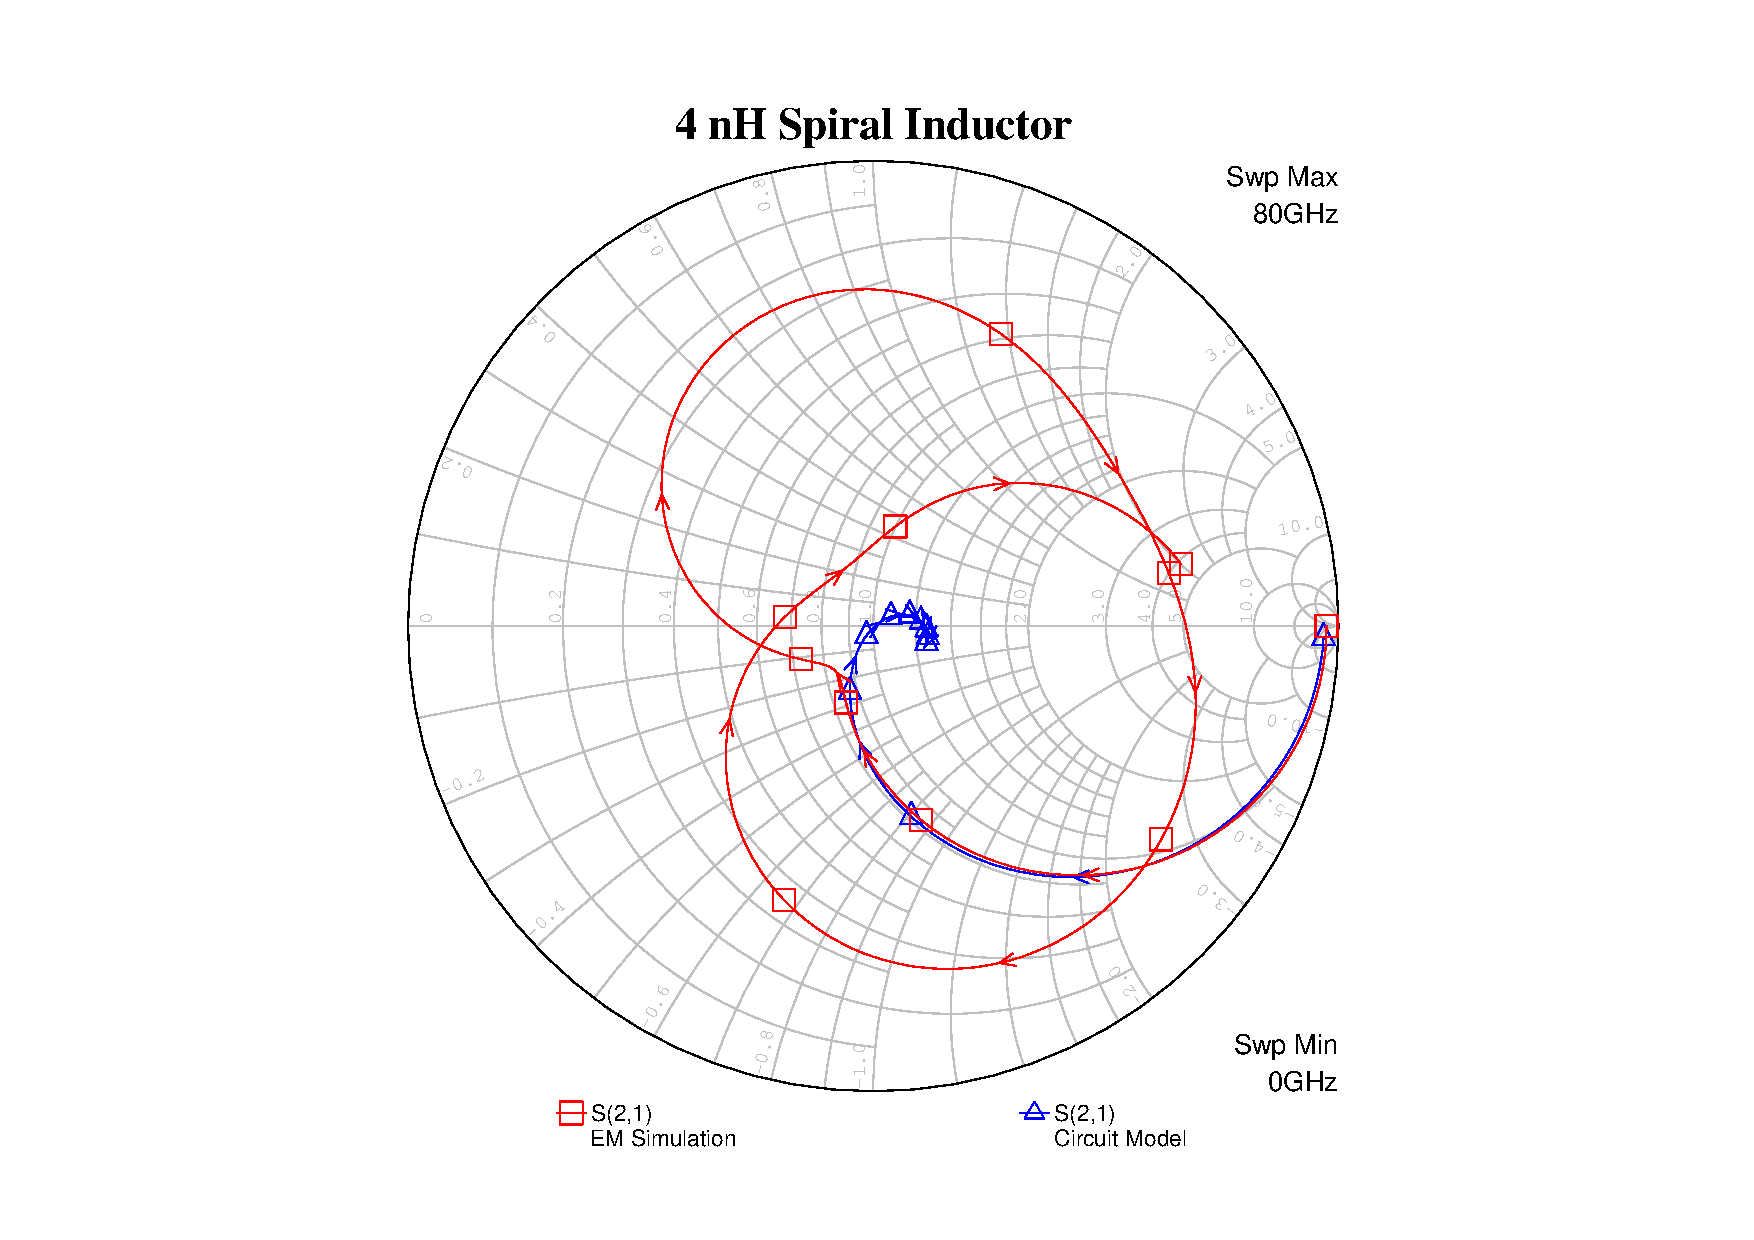
\includegraphics[width=1.0\textwidth]{fig/emsim/inductor4smith}
			\includesmith{0.9\textwidth}{fig/emsim/inductor4smith}
			\caption[EM simulation of the UMS PPH25 spiral inductor.]{Comparison of S$_{21}$ between the electric model of the PPH25 spiral inductor and its EM simulation. For low frequencies the results are approximately the same. The electric circuit model is not trustworthy above $\sim$\unit[12]{GHz}, for a \unit[4]{nH} inductance.}\label{fig:emsiminductor4}
		\end{figure}

		\begin{figure}[hpt!]
			\centering
			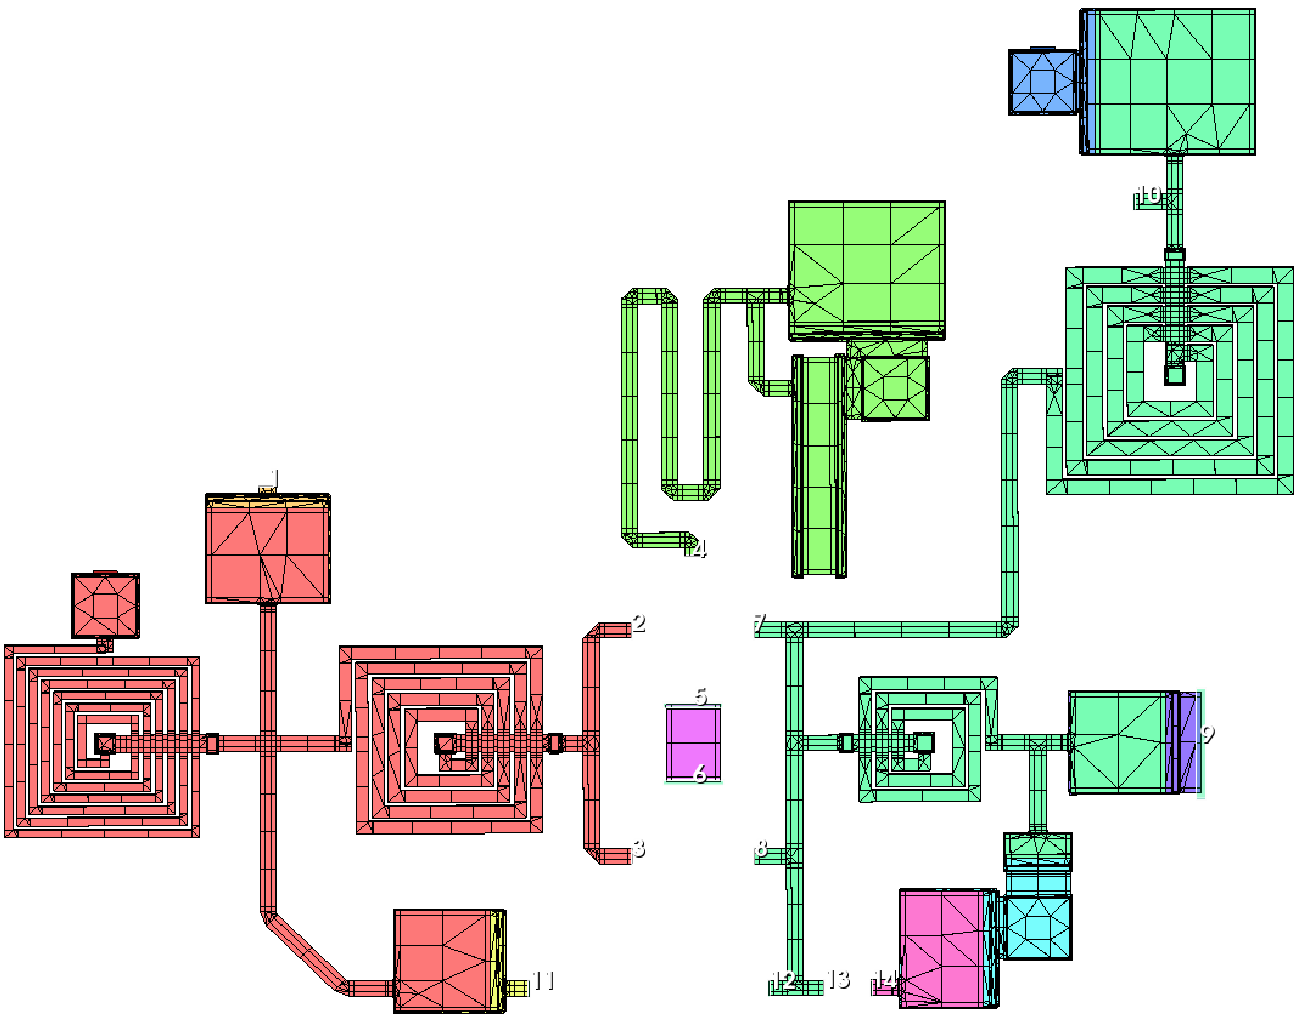
\includegraphics[width=0.7\textwidth]{fig/emsim/if2mesh}
			\caption[EM mesh of amplifier IF2.]{Meshed EM structure of the passive components in amplifier IF2. Bias, input, output and active components (including the GaAs resistors) are connected with edge ports. Areas of the same colour are DC-connected.}\label{fig:if2mesh}
		\end{figure}
